% Codigo do grafico de trajetorias dos 5 primeiros participantes (Exp 3)
\begin{figure}[H]
\centering
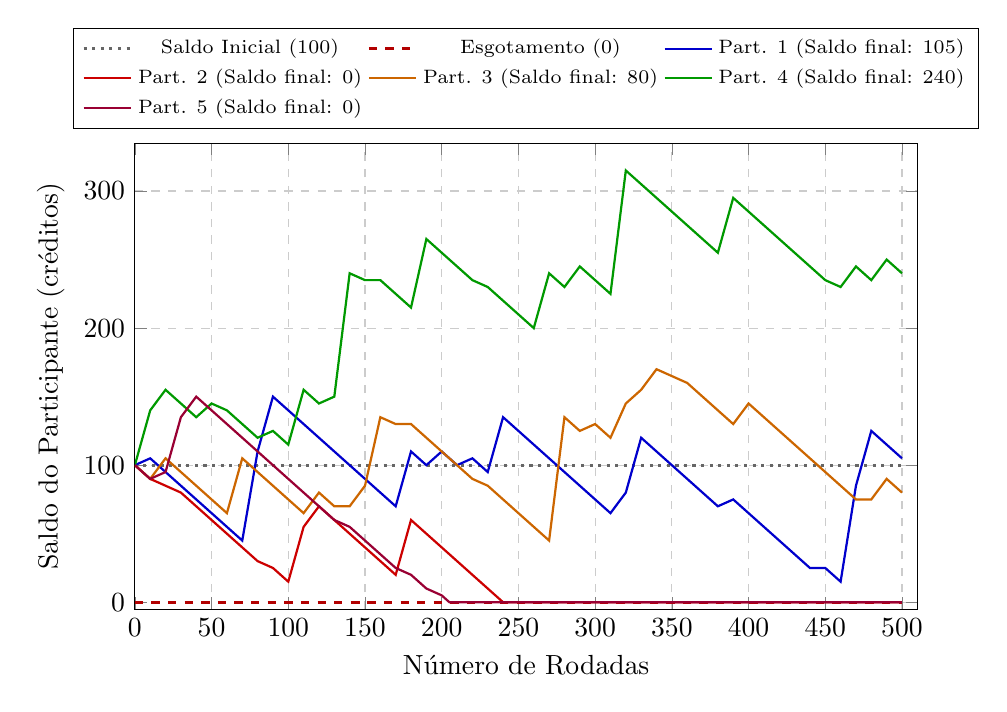
\begin{tikzpicture}
\begin{axis}[
    width=0.95\textwidth,
    height=7.5cm,
    xlabel={Número de Rodadas},
    ylabel={Saldo do Participante (créditos)},
    xmin=0, xmax=510,
    ymin=-5, ymax=335,
    legend style={at={(0.5,1.03)}, anchor=south, legend columns=3, font=\scriptsize},
    grid=major,
    major grid style={dashed, gray!40}
]

% Linha de referencia: Saldo Inicial 100
\addplot[gray!80!black, dotted, line width=1.1pt, domain=0:500] {100};
\addlegendentry{Saldo Inicial ($100$)}
% Linha de esgotamento: 0
\addplot[red!70!black, dashed, line width=1.0pt, domain=0:500] {0};
\addlegendentry{Esgotamento ($0$)}

% Participante 1
\addplot[blue!80!black, thick] coordinates {
    (0, 100.0)
    (10, 105.0)
    (20, 95.0)
    (30, 85.0)
    (40, 75.0)
    (50, 65.0)
    (60, 55.0)
    (70, 45.0)
    (80, 110.0)
    (90, 150.0)
    (100, 140.0)
    (110, 130.0)
    (120, 120.0)
    (130, 110.0)
    (140, 100.0)
    (150, 90.0)
    (160, 80.0)
    (170, 70.0)
    (180, 110.0)
    (190, 100.0)
    (200, 110.0)
    (210, 100.0)
    (220, 105.0)
    (230, 95.0)
    (240, 135.0)
    (250, 125.0)
    (260, 115.0)
    (270, 105.0)
    (280, 95.0)
    (290, 85.0)
    (300, 75.0)
    (310, 65.0)
    (320, 80.0)
    (330, 120.0)
    (340, 110.0)
    (350, 100.0)
    (360, 90.0)
    (370, 80.0)
    (380, 70.0)
    (390, 75.0)
    (400, 65.0)
    (410, 55.0)
    (420, 45.0)
    (430, 35.0)
    (440, 25.0)
    (450, 25.0)
    (460, 15.0)
    (470, 85.0)
    (480, 125.0)
    (490, 115.0)
    (500, 105.0)
};
\addlegendentry{Part. 1 (Saldo final: 105)}

% Participante 2
\addplot[red!80!black, thick] coordinates {
    (0, 100.0)
    (10, 90.0)
    (20, 85.0)
    (30, 80.0)
    (40, 70.0)
    (50, 60.0)
    (60, 50.0)
    (70, 40.0)
    (80, 30.0)
    (90, 25.0)
    (100, 15.0)
    (110, 55.0)
    (120, 70.0)
    (130, 60.0)
    (140, 50.0)
    (150, 40.0)
    (160, 30.0)
    (170, 20.0)
    (180, 60.0)
    (190, 50.0)
    (200, 40.0)
    (210, 30.0)
    (220, 20.0)
    (230, 10.0)
    (240, 0.0)
    (250, 0.0)
    (300, 0.0)
    (350, 0.0)
    (400, 0.0)
    (450, 0.0)
    (500, 0.0)
};
\addlegendentry{Part. 2 (Saldo final: 0)}

% Participante 3
\addplot[orange!80!black, thick] coordinates {
    (0, 100.0)
    (10, 90.0)
    (20, 105.0)
    (30, 95.0)
    (40, 85.0)
    (50, 75.0)
    (60, 65.0)
    (70, 105.0)
    (80, 95.0)
    (90, 85.0)
    (100, 75.0)
    (110, 65.0)
    (120, 80.0)
    (130, 70.0)
    (140, 70.0)
    (150, 85.0)
    (160, 135.0)
    (170, 130.0)
    (180, 130.0)
    (190, 120.0)
    (200, 110.0)
    (210, 100.0)
    (220, 90.0)
    (230, 85.0)
    (240, 75.0)
    (250, 65.0)
    (260, 55.0)
    (270, 45.0)
    (280, 135.0)
    (290, 125.0)
    (300, 130.0)
    (310, 120.0)
    (320, 145.0)
    (330, 155.0)
    (340, 170.0)
    (350, 165.0)
    (360, 160.0)
    (370, 150.0)
    (380, 140.0)
    (390, 130.0)
    (400, 145.0)
    (410, 135.0)
    (420, 125.0)
    (430, 115.0)
    (440, 105.0)
    (450, 95.0)
    (460, 85.0)
    (470, 75.0)
    (480, 75.0)
    (490, 90.0)
    (500, 80.0)
};
\addlegendentry{Part. 3 (Saldo final: 80)}

% Participante 4
\addplot[green!60!black, thick] coordinates {
    (0, 100.0)
    (10, 140.0)
    (20, 155.0)
    (30, 145.0)
    (40, 135.0)
    (50, 145.0)
    (60, 140.0)
    (70, 130.0)
    (80, 120.0)
    (90, 125.0)
    (100, 115.0)
    (110, 155.0)
    (120, 145.0)
    (130, 150.0)
    (140, 240.0)
    (150, 235.0)
    (160, 235.0)
    (170, 225.0)
    (180, 215.0)
    (190, 265.0)
    (200, 255.0)
    (210, 245.0)
    (220, 235.0)
    (230, 230.0)
    (240, 220.0)
    (250, 210.0)
    (260, 200.0)
    (270, 240.0)
    (280, 230.0)
    (290, 245.0)
    (300, 235.0)
    (310, 225.0)
    (320, 315.0)
    (330, 305.0)
    (340, 295.0)
    (350, 285.0)
    (360, 275.0)
    (370, 265.0)
    (380, 255.0)
    (390, 295.0)
    (400, 285.0)
    (410, 275.0)
    (420, 265.0)
    (430, 255.0)
    (440, 245.0)
    (450, 235.0)
    (460, 230.0)
    (470, 245.0)
    (480, 235.0)
    (490, 250.0)
    (500, 240.0)
};
\addlegendentry{Part. 4 (Saldo final: 240)}

% Participante 5
\addplot[purple!80!black, thick] coordinates {
    (0, 100.0)
    (10, 90.0)
    (20, 95.0)
    (30, 135.0)
    (40, 150.0)
    (50, 140.0)
    (60, 130.0)
    (70, 120.0)
    (80, 110.0)
    (90, 100.0)
    (100, 90.0)
    (110, 80.0)
    (120, 70.0)
    (130, 60.0)
    (140, 55.0)
    (150, 45.0)
    (160, 35.0)
    (170, 25.0)
    (180, 20.0)
    (190, 10.0)
    (200, 5.0)
    (205, 0.0)
    (210, 0.0)
    (260, 0.0)
    (310, 0.0)
    (360, 0.0)
    (410, 0.0)
    (460, 0.0)
    (500, 0.0)
};
\addlegendentry{Part. 5 (Saldo final: 0)}

\end{axis}
\end{tikzpicture}
\caption{Evolução do saldo dos cinco primeiros participantes virtuais ao longo de até $500$ rodadas (semente 42). Nota-se que os participantes 2 e 5 sofreram esgotamento precoce (ruína do jogador), o participante 3 terminou em perda sem ruína, enquanto os participantes 1 e 4 encerraram com lucro.}
\label{fig:exp3_trajetorias_5}
\end{figure}
